\clearpage
\subsection{Expressions (with Arrays)} % (fold)
\label{sub:expressions_with_arrays_}

Expressions allow you to read values from the elements of an array. To get an elements value you must supply the name of the array, and the index of the element you want to read.

\begin{figure}[h]
   \centering
   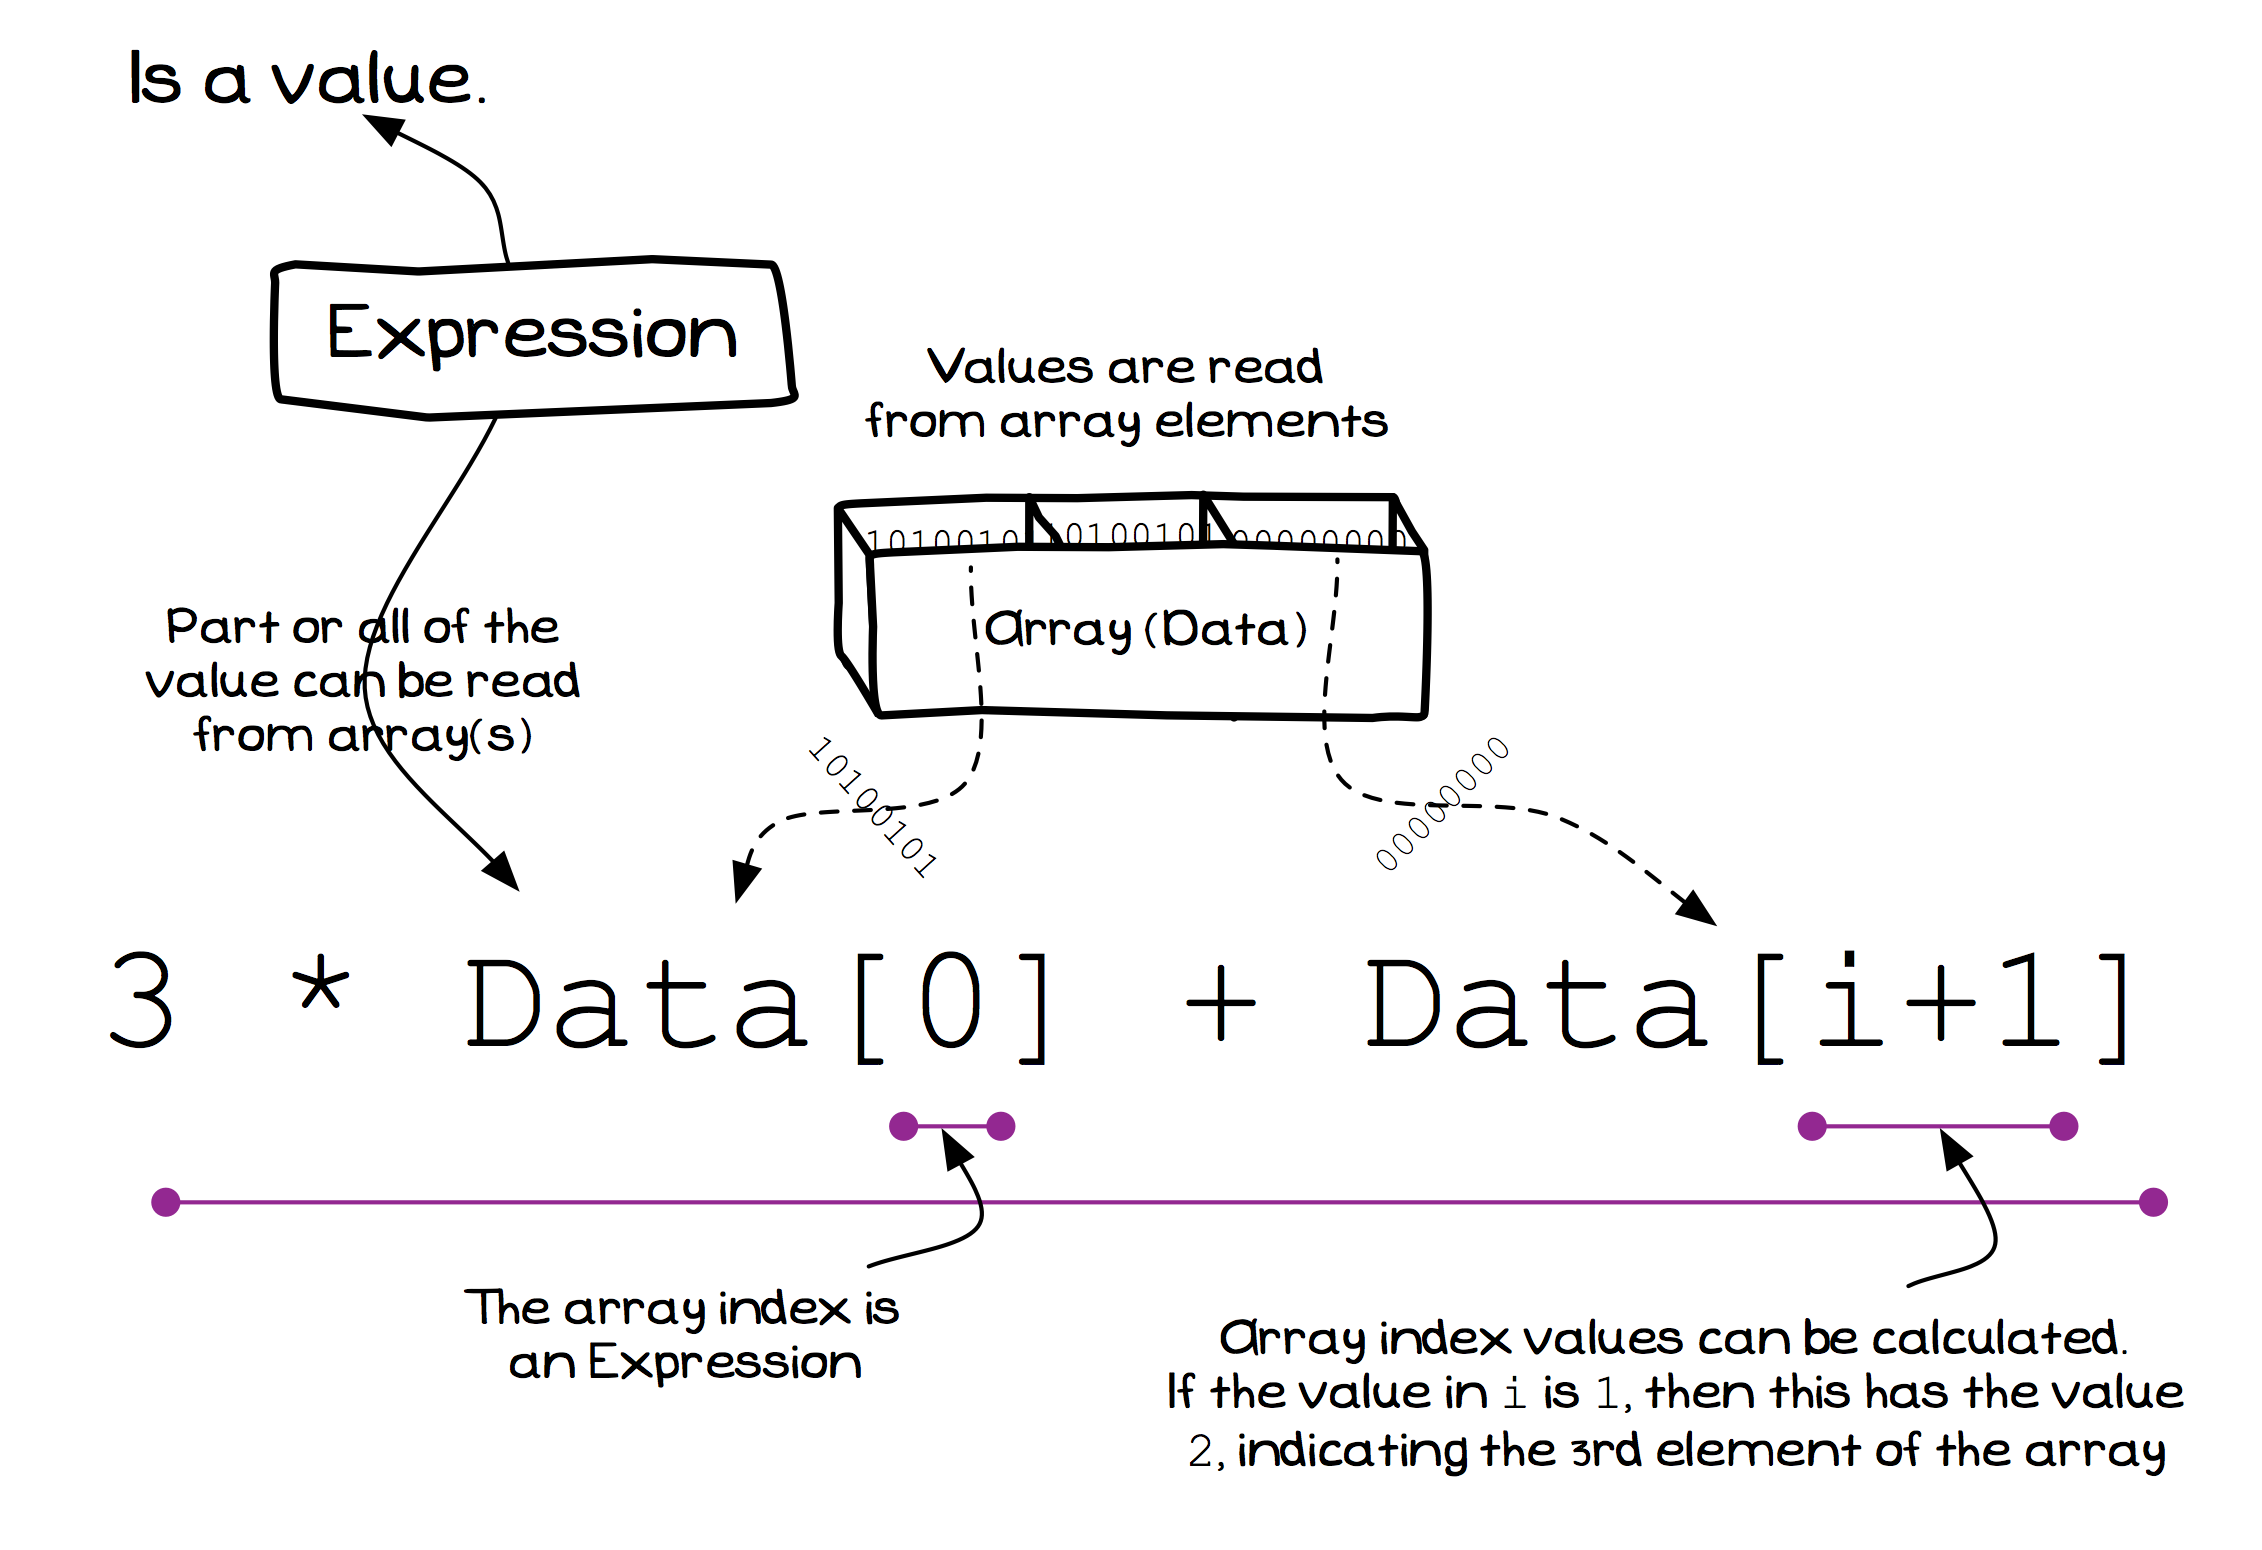
\includegraphics[width=\textwidth]{./topics/arrays/diagrams/ExpressionWithArray} 
   \caption{You can read the values back from an array}
   \label{fig:expression-with-arrays}
\end{figure}

\mynote {
\begin{itemize}
  \item Expression is the \textbf{term} given to the code that calculates values within your Statements.
  \item You can read the values of elements of an array in an expression.
  \item The index values used to access the individual elements of an array are expressions themselves.
  \item Arrays are similar to variables in expressions, the expression reads the value from the element of the array.
  \item The index you supply determine which value is read.
\end{itemize}
}

% subsection expressions_with_arrays_ (end)